\documentclass[a4paper,14pt]{extreport}
\usepackage[left=1.5cm,right=1.5cm,
    top=1.5cm,bottom=2cm,bindingoffset=0cm]{geometry}
\usepackage{scrextend}
\usepackage[T1,T2A]{fontenc}
\usepackage[utf8]{inputenc}
\usepackage[english,russian,ukrainian]{babel}
\usepackage{tabularx}
\usepackage{amssymb}
\usepackage{color}
\usepackage{amsmath}
\usepackage{mathrsfs}
\usepackage{listings}
\usepackage{graphicx}
\graphicspath{ {./images/} }
\usepackage{lipsum}
\usepackage{xcolor}
\usepackage{hyperref}

\usepackage{tcolorbox}
\usepackage{tikz}
\usepackage[framemethod=TikZ]{mdframed}
\usepackage{wrapfig,boxedminipage,lipsum}
\mdfdefinestyle{MyFrame}{%
linecolor=blue,outerlinewidth=2pt,roundcorner=20pt,innertopmargin=\baselineskip,innerbottommargin=\baselineskip,innerrightmargin=20pt,innerleftmargin=20pt,backgroundcolor=gray!50!white}
 \usepackage{csvsimple}
 \usepackage{supertabular}
\usepackage{pdflscape}
\usepackage{fancyvrb}
%\usepackage{comment}
\definecolor{ggreen}{rgb}{0.,1,0}
\definecolor{rred}{rgb}{1,0.1,0.1}
\usepackage{array,tabularx}
\usepackage{colortbl}

\usepackage{varwidth}
\tcbuselibrary{skins}
\usepackage{fancybox}




\usepackage{float}
\usepackage{wrapfig}
\usepackage{framed}





\begin{document}
\renewcommand{\bibname}{Список використаної літератури}
\pagecolor{white}
\begin{titlepage}
  \begin{center}
    \large
    Національний технічний університет України \\ "Київський політехнічний інститут імені Ігоря Сікорського"


    Факультет Електроніки

    Кафедра мікроелектроніки
    \vfill

    \textsc{ЗВІТ}\\

    {\Large Про виконання домашньої контрольної роботи\\
      з дисципліни: «Фізика напівпровідніків»\\[1cm]



    }
  \bigskip
\end{center}
\vfill

\newlength{\ML}
\settowidth{\ML}{«\underline{\hspace{0.4cm}}» \underline{\hspace{2cm}}}
\hfill
\begin{minipage}{1\textwidth}
Виконавець:\\
Студент 3-го курсу \hspace{4cm} $\underset{\text{(підпис)}}{\underline{\hspace{0.2\textwidth}}}$  \hspace{1cm}А.\,Р.~Півчук\\
\vspace{1cm}

Перевірив: \hspace{6.1cm} $\underset{\text{(підпис)}}{\underline{\hspace{0.2\textwidth}}}$  \hspace{1cm}Т.\,Ю.~Обухова\\

\end{minipage}

\vfill

\begin{center}
2020
\end{center}
\end{titlepage}


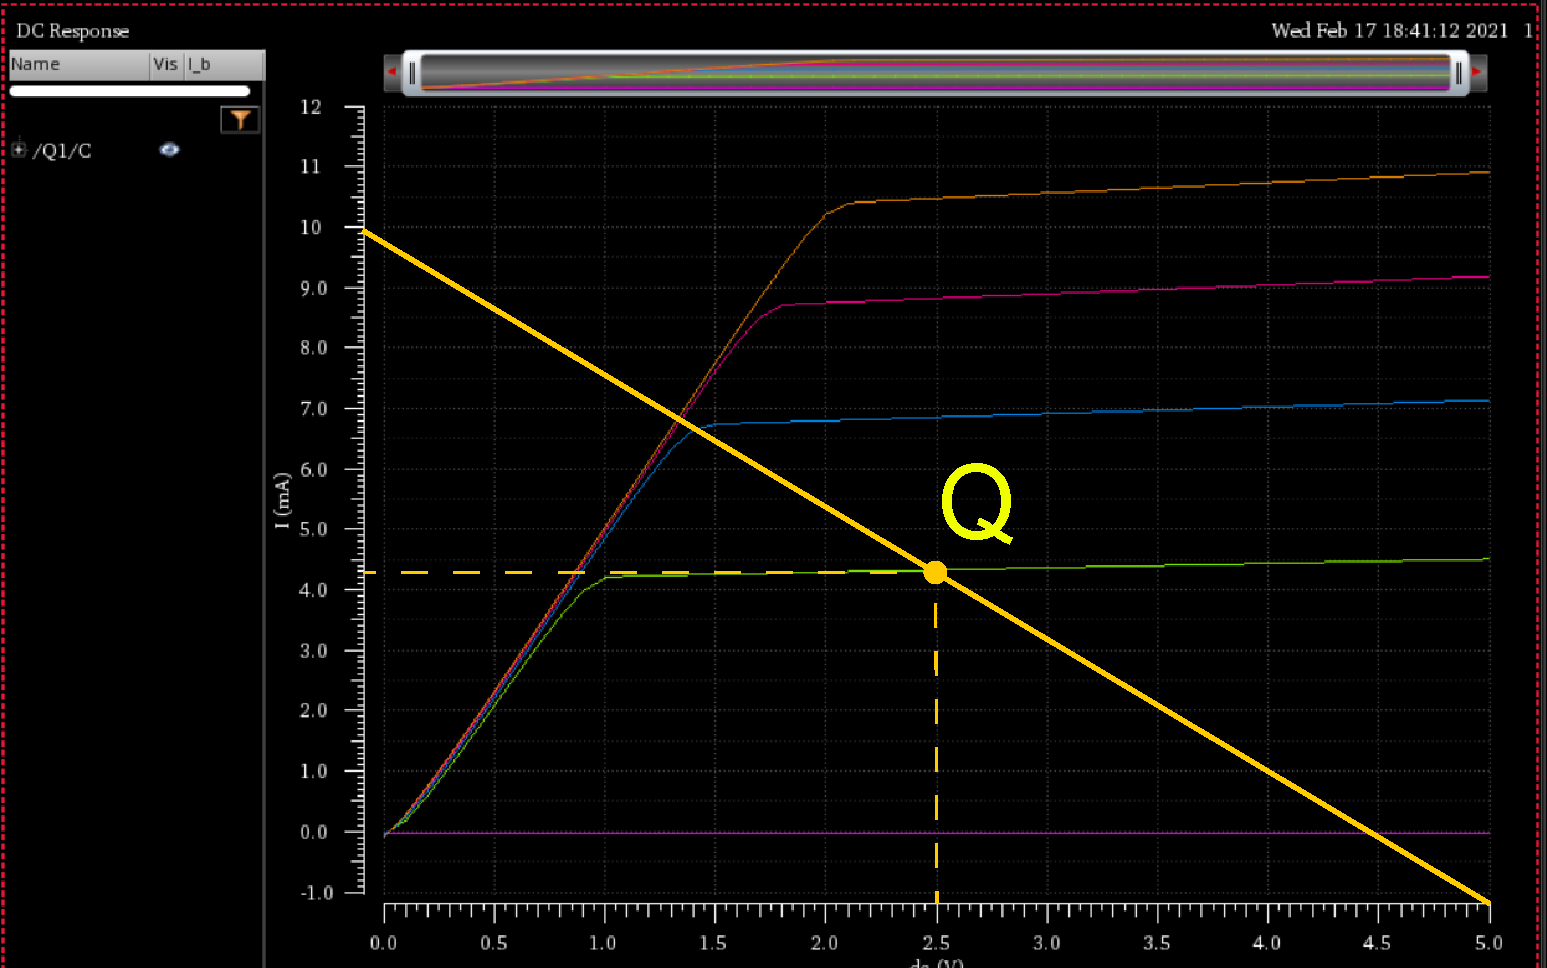
\includegraphics[scale=0.5]{1.png}

\begin{center}
  \textbf{Завдання 1}
\end{center}
\begin{equation}
  R_{H} =\dfrac{1}{qn}
\end{equation}

\begin{equation}
  n = \dfrac{1}{qR_{H}}
  = \dfrac{1}{1,6\cdot 10^{-19} \cdot 2,1\cdot 10^{-3}}
  =  2.976\cdot 10^{21} \text{ м}^{-3}
\end{equation}


\begin{center}
  \textbf{Завдання 2}
\end{center}

\begin{equation}
f_{\text{рез}} = \dfrac{c}{\lambda_{\text{рез}}}
=\dfrac{3\cdot 10^{8}}{11,5\cdot 10^{-6}}
= 2,6\cdot 10^{13} \text{ Гц}
\end{equation}

\begin{equation}
m* = \dfrac{e^2n^+}{\varepsilon\varepsilon_0f_{\text{рез}}^2}
= \dfrac{(1,6\cdot10^{-19})^2 \cdot 2\cdot10^{25}}{11,7\cdot8,8\cdot10^{-12} \cdot (2,6\cdot 10^{13})^2}
= 7.307 \cdot 10^{-30} \text{ кг}
\end{equation}

\begin{center}
  \textbf{Завдання 3}
\end{center}

\begin{equation}
j_s = qn\sqrt{\dfrac{h\omega_0}{m*}} = 1,6\cdot10^{-19}\cdot  2.976\cdot 10^{21}\sqrt{\dfrac{0,088\cdot 10^{-19}}{7.307 \cdot 10^{-30}}}
= 1.652\cdot 10^{7}  \dfrac{A}{\text{м}^2}
\end{equation}





\end{document}
